\documentclass[tikz,border=6pt]{standalone}
\usepackage[T1]{fontenc}
\usepackage[scaled=0.92]{helvet}
\usepackage{amsmath,amssymb}
\usepackage{tikz}
\usetikzlibrary{arrows.meta,positioning,shapes.geometric,shapes.misc,calc,fit,backgrounds}

\begin{document}
\sffamily
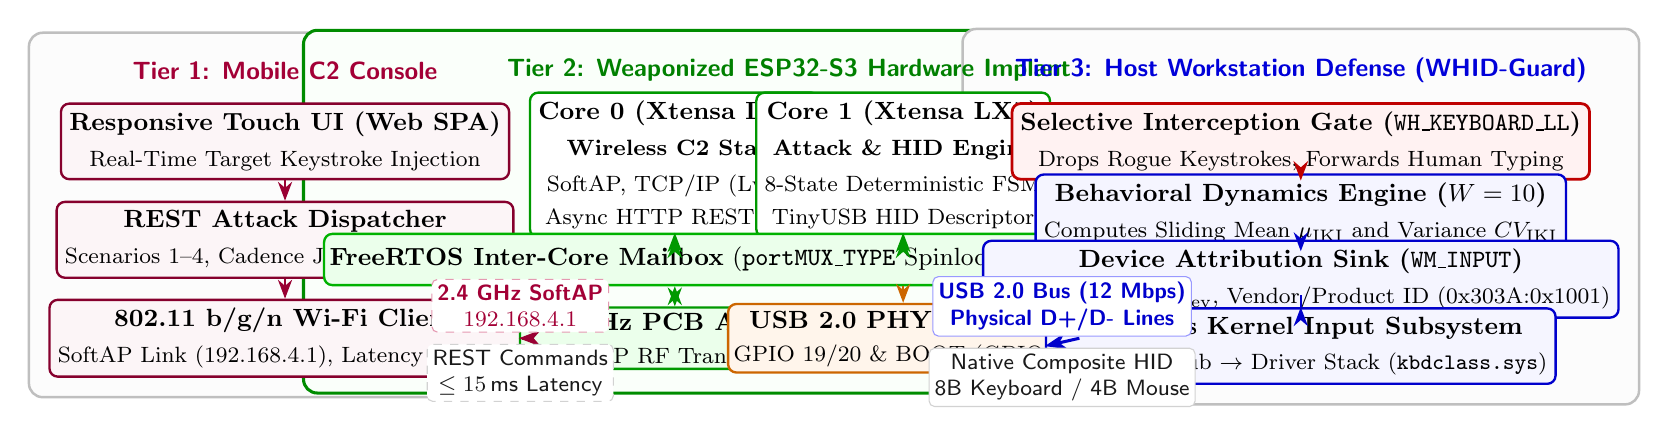
\begin{tikzpicture}[
    >=Stealth,
    font=\small,
    % Outer Container Styles
    tier_box/.style={
        rectangle,
        rounded corners=5pt,
        draw=gray!50,
        line width=0.9pt,
        fill=gray!2,
        inner sep=7pt
    },
    % Module Card Styles
    c2_card/.style={
        rectangle,
        rounded corners=3pt,
        draw=purple!70!black,
        line width=0.85pt,
        fill=purple!4!white,
        minimum width=4.5cm,
        minimum height=0.92cm,
        inner sep=3pt,
        align=center
    },
    soc_chip/.style={
        rectangle,
        rounded corners=5pt,
        draw=green!55!black,
        line width=1.1pt,
        fill=green!2!white,
        inner sep=7pt
    },
    core_box/.style={
        rectangle,
        rounded corners=3pt,
        draw=green!60!black,
        line width=0.85pt,
        fill=white,
        minimum width=2.65cm,
        minimum height=1.55cm,
        inner sep=3pt,
        align=center
    },
    ipc_box/.style={
        rectangle,
        rounded corners=3pt,
        draw=green!70!black,
        line width=0.85pt,
        fill=green!8!white,
        minimum width=5.5cm,
        minimum height=0.65cm,
        inner sep=2pt,
        align=center
    },
    hw_box/.style={
        rectangle,
        rounded corners=3pt,
        draw=orange!80!black,
        line width=0.85pt,
        fill=orange!8!white,
        minimum width=2.65cm,
        minimum height=0.72cm,
        inner sep=2pt,
        align=center
    },
    host_card/.style={
        rectangle,
        rounded corners=3pt,
        draw=blue!80!black,
        line width=0.85pt,
        fill=blue!4!white,
        minimum width=4.7cm,
        minimum height=0.82cm,
        inner sep=3pt,
        align=center
    },
    gate_card/.style={
        rectangle,
        rounded corners=3pt,
        draw=red!75!black,
        line width=1.0pt,
        fill=red!5!white,
        minimum width=4.7cm,
        minimum height=0.82cm,
        inner sep=3pt,
        align=center
    },
    % Badges
    lbl/.style={
        font=\sffamily\footnotesize,
        fill=white,
        draw=gray!35,
        line width=0.4pt,
        rounded corners=2pt,
        inner sep=2pt,
        align=center,
        text=black!90
    },
    lbl_purple/.style={
        font=\sffamily\footnotesize\bfseries,
        fill=white,
        draw=purple!40,
        line width=0.4pt,
        rounded corners=2pt,
        inner sep=2pt,
        align=center,
        text=purple!85!black
    },
    lbl_green/.style={
        font=\sffamily\footnotesize\bfseries,
        fill=white,
        draw=green!50!black,
        line width=0.4pt,
        rounded corners=2pt,
        inner sep=2pt,
        align=center,
        text=green!60!black
    },
    lbl_blue/.style={
        font=\sffamily\footnotesize\bfseries,
        fill=white,
        draw=blue!40,
        line width=0.4pt,
        rounded corners=2pt,
        inner sep=2pt,
        align=center,
        text=blue!80!black
    }
]

% ==============================================================================
% TIER 1: Out-of-Band Wireless Mobile Controller (C2) (x = 2.4)
% ==============================================================================
\node[font=\sffamily\bfseries\small, text=purple!85!black] (t1_title) at (2.4, 1.85) {Tier 1: Mobile C2 Console};

\node[c2_card] (c2_web)  at (2.4, 0.95) {\textbf{Responsive Touch UI (Web SPA)}\\[2pt]\footnotesize Real-Time Target Keystroke Injection};

\node[c2_card] (c2_api)  at (2.4, -0.30) {\textbf{REST Attack Dispatcher}\\[2pt]\footnotesize Scenarios 1--4, Cadence Jitter, Abort $\phi_{\text{stop}}$};

\node[c2_card] (c2_wifi) at (2.4, -1.55) {\textbf{802.11 b/g/n Wi-Fi Client}\\[2pt]\footnotesize SoftAP Link ($192.168.4.1$), Latency $\le 15$\,ms};

\draw[->, line width=0.85pt, draw=purple!80!black] (c2_web.south) -- (c2_api.north);
\draw[->, line width=0.85pt, draw=purple!80!black] (c2_api.south) -- (c2_wifi.north);

\begin{scope}[on background layer]
    \node[tier_box, fit=(t1_title) (c2_web) (c2_api) (c2_wifi)] (tier1_bg) {};
\end{scope}

% ==============================================================================
% TIER 2: Embedded ESP32-S3 Hardware Implant (x = 8.8)
% ==============================================================================
\node[font=\sffamily\bfseries\small, text=green!50!black] (t2_title) at (8.8, 1.85) {Tier 2: Weaponized ESP32-S3 Hardware Implant};

% Core 0 Box (Left, x = 7.35, y = 0.65)
\node[core_box] (core0) at (7.35, 0.65) {
    \textbf{Core 0 (Xtensa LX7)}\\[2pt]
    \footnotesize\textbf{Wireless C2 Stack}\\[2pt]
    \footnotesize SoftAP, TCP/IP (LwIP)\\[1pt]
    \footnotesize Async HTTP REST API
};

% Core 1 Box (Right, x = 10.25, y = 0.65)
\node[core_box] (core1) at (10.25, 0.65) {
    \textbf{Core 1 (Xtensa LX7)}\\[2pt]
    \footnotesize\textbf{Attack \& HID Engine}\\[2pt]
    \footnotesize 8-State Deterministic FSM\\[1pt]
    \footnotesize TinyUSB HID Descriptor
};

% Spinlock Shared Mailbox (Center, y = -0.55)
\node[ipc_box] (ipc) at (8.8, -0.55) {
    \textbf{FreeRTOS Inter-Core Mailbox} (\texttt{portMUX\_TYPE} Spinlock, Shared Ring Buffer)
};

\draw[<->, line width=0.9pt, draw=green!60!black] (core0.south) -- (core0.south |- ipc.north);
\draw[<->, line width=0.9pt, draw=green!60!black] (core1.south) -- (core1.south |- ipc.north);

% Hardware Peripherals (Bottom, y = -1.55)
\node[hw_box, draw=green!60!black, fill=green!8!white] (ant_hw) at (7.35, -1.55) {
    \textbf{2.4 GHz PCB Antenna}\\[1pt]\footnotesize SoftAP RF Transceiver
};

\node[hw_box] (usb_hw) at (10.25, -1.55) {
    \textbf{USB 2.0 PHY (D+/D-)}\\[1pt]\footnotesize GPIO 19/20 \& BOOT (GPIO 0)
};

\draw[<->, line width=0.85pt, draw=green!60!black] (ant_hw.north) -- (ant_hw.north |- ipc.south);
\draw[->, line width=0.85pt, draw=orange!80!black] (ipc.south -| usb_hw.north) -- (usb_hw.north);

\begin{scope}[on background layer]
    \node[soc_chip, fit=(t2_title) (core0) (core1) (ipc) (ant_hw) (usb_hw)] (soc_bg) {};
\end{scope}

% ==============================================================================
% TIER 3: Host Workstation & WHID-Guard Defense (x = 15.3)
% ==============================================================================
\node[font=\sffamily\bfseries\small, text=blue!85!black] (t3_title) at (15.3, 1.85) {Tier 3: Host Workstation Defense (WHID-Guard)};

\node[gate_card] (host_gate) at (15.3, 0.95) {
    \textbf{Selective Interception Gate (\texttt{WH\_KEYBOARD\_LL})}\\[2pt]
    \footnotesize Drops Rogue Keystrokes, Forwards Human Typing
};

\node[host_card] (host_engine) at (15.3, 0.05) {
    \textbf{Behavioral Dynamics Engine ($W=10$)}\\[2pt]
    \footnotesize Computes Sliding Mean $\mu_{\text{IKI}}$ and Variance $CV_{\text{IKI}}$
};

\node[host_card] (host_raw) at (15.3, -0.80) {
    \textbf{Device Attribution Sink (\texttt{WM\_INPUT})}\\[2pt]
    \footnotesize Resolves Handle $h_{\text{dev}}$, Vendor/Product ID (0x303A:0x1001)
};

\node[host_card] (host_kernel) at (15.3, -1.65) {
    \textbf{Windows Kernel Input Subsystem}\\[2pt]
    \footnotesize Root USB Hub $\rightarrow$ Driver Stack (\texttt{kbdclass.sys})
};

% Ascending defense pipeline inside Tier 3
\draw[->, line width=0.85pt, draw=blue!80!black] (host_kernel.north) -- (host_raw.north |- host_kernel.north);
\draw[->, line width=0.85pt, draw=blue!80!black] (host_raw.north) -- (host_engine.south);
\draw[->, line width=0.9pt, draw=red!75!black] (host_engine.north) -- (host_gate.south);

\begin{scope}[on background layer]
    \node[tier_box, fit=(t3_title) (host_gate) (host_engine) (host_raw) (host_kernel)] (tier3_bg) {};
\end{scope}

% ==============================================================================
% INTER-TIER CONNECTIONS (Clean, Straight Horizontal Flows!)
% ==============================================================================
% Tier 1 (Wi-Fi) -> Tier 2 (PCB Antenna) at y = -1.55
\draw[->, line width=1.1pt, draw=purple!80!black, dashed] (c2_wifi.east) -- (ant_hw.west)
    node[pos=0.5, above=2pt, lbl_purple] {2.4 GHz SoftAP\\$192.168.4.1$}
    node[pos=0.5, below=2pt, lbl] {REST Commands\\$\le 15$\,ms Latency};

% Tier 2 (USB 2.0 PHY) -> Tier 3 (Kernel / USB Hub) at y = -1.65
\draw[->, line width=1.1pt, draw=blue!80!black] (usb_hw.east) -- (host_kernel.west)
    node[pos=0.5, above=2pt, lbl_blue] {USB 2.0 Bus (12 Mbps)\\Physical D+/D- Lines}
    node[pos=0.5, below=2pt, lbl] {Native Composite HID\\8B Keyboard / 4B Mouse};

\end{tikzpicture}
\end{document}
